% Options for packages loaded elsewhere
\PassOptionsToPackage{unicode}{hyperref}
\PassOptionsToPackage{hyphens}{url}
%
\documentclass[
]{article}
\usepackage{amsmath,amssymb}
\usepackage{iftex}
\ifPDFTeX
  \usepackage[T1]{fontenc}
  \usepackage[utf8]{inputenc}
  \usepackage{textcomp} % provide euro and other symbols
\else % if luatex or xetex
  \usepackage{unicode-math} % this also loads fontspec
  \defaultfontfeatures{Scale=MatchLowercase}
  \defaultfontfeatures[\rmfamily]{Ligatures=TeX,Scale=1}
\fi
\usepackage{lmodern}
\ifPDFTeX\else
  % xetex/luatex font selection
\fi
% Use upquote if available, for straight quotes in verbatim environments
\IfFileExists{upquote.sty}{\usepackage{upquote}}{}
\IfFileExists{microtype.sty}{% use microtype if available
  \usepackage[]{microtype}
  \UseMicrotypeSet[protrusion]{basicmath} % disable protrusion for tt fonts
}{}
\makeatletter
\@ifundefined{KOMAClassName}{% if non-KOMA class
  \IfFileExists{parskip.sty}{%
    \usepackage{parskip}
  }{% else
    \setlength{\parindent}{0pt}
    \setlength{\parskip}{6pt plus 2pt minus 1pt}}
}{% if KOMA class
  \KOMAoptions{parskip=half}}
\makeatother
\usepackage{xcolor}
\usepackage[margin=1in]{geometry}
\usepackage{color}
\usepackage{fancyvrb}
\newcommand{\VerbBar}{|}
\newcommand{\VERB}{\Verb[commandchars=\\\{\}]}
\DefineVerbatimEnvironment{Highlighting}{Verbatim}{commandchars=\\\{\}}
% Add ',fontsize=\small' for more characters per line
\usepackage{framed}
\definecolor{shadecolor}{RGB}{248,248,248}
\newenvironment{Shaded}{\begin{snugshade}}{\end{snugshade}}
\newcommand{\AlertTok}[1]{\textcolor[rgb]{0.94,0.16,0.16}{#1}}
\newcommand{\AnnotationTok}[1]{\textcolor[rgb]{0.56,0.35,0.01}{\textbf{\textit{#1}}}}
\newcommand{\AttributeTok}[1]{\textcolor[rgb]{0.13,0.29,0.53}{#1}}
\newcommand{\BaseNTok}[1]{\textcolor[rgb]{0.00,0.00,0.81}{#1}}
\newcommand{\BuiltInTok}[1]{#1}
\newcommand{\CharTok}[1]{\textcolor[rgb]{0.31,0.60,0.02}{#1}}
\newcommand{\CommentTok}[1]{\textcolor[rgb]{0.56,0.35,0.01}{\textit{#1}}}
\newcommand{\CommentVarTok}[1]{\textcolor[rgb]{0.56,0.35,0.01}{\textbf{\textit{#1}}}}
\newcommand{\ConstantTok}[1]{\textcolor[rgb]{0.56,0.35,0.01}{#1}}
\newcommand{\ControlFlowTok}[1]{\textcolor[rgb]{0.13,0.29,0.53}{\textbf{#1}}}
\newcommand{\DataTypeTok}[1]{\textcolor[rgb]{0.13,0.29,0.53}{#1}}
\newcommand{\DecValTok}[1]{\textcolor[rgb]{0.00,0.00,0.81}{#1}}
\newcommand{\DocumentationTok}[1]{\textcolor[rgb]{0.56,0.35,0.01}{\textbf{\textit{#1}}}}
\newcommand{\ErrorTok}[1]{\textcolor[rgb]{0.64,0.00,0.00}{\textbf{#1}}}
\newcommand{\ExtensionTok}[1]{#1}
\newcommand{\FloatTok}[1]{\textcolor[rgb]{0.00,0.00,0.81}{#1}}
\newcommand{\FunctionTok}[1]{\textcolor[rgb]{0.13,0.29,0.53}{\textbf{#1}}}
\newcommand{\ImportTok}[1]{#1}
\newcommand{\InformationTok}[1]{\textcolor[rgb]{0.56,0.35,0.01}{\textbf{\textit{#1}}}}
\newcommand{\KeywordTok}[1]{\textcolor[rgb]{0.13,0.29,0.53}{\textbf{#1}}}
\newcommand{\NormalTok}[1]{#1}
\newcommand{\OperatorTok}[1]{\textcolor[rgb]{0.81,0.36,0.00}{\textbf{#1}}}
\newcommand{\OtherTok}[1]{\textcolor[rgb]{0.56,0.35,0.01}{#1}}
\newcommand{\PreprocessorTok}[1]{\textcolor[rgb]{0.56,0.35,0.01}{\textit{#1}}}
\newcommand{\RegionMarkerTok}[1]{#1}
\newcommand{\SpecialCharTok}[1]{\textcolor[rgb]{0.81,0.36,0.00}{\textbf{#1}}}
\newcommand{\SpecialStringTok}[1]{\textcolor[rgb]{0.31,0.60,0.02}{#1}}
\newcommand{\StringTok}[1]{\textcolor[rgb]{0.31,0.60,0.02}{#1}}
\newcommand{\VariableTok}[1]{\textcolor[rgb]{0.00,0.00,0.00}{#1}}
\newcommand{\VerbatimStringTok}[1]{\textcolor[rgb]{0.31,0.60,0.02}{#1}}
\newcommand{\WarningTok}[1]{\textcolor[rgb]{0.56,0.35,0.01}{\textbf{\textit{#1}}}}
\usepackage{longtable,booktabs,array}
\usepackage{calc} % for calculating minipage widths
% Correct order of tables after \paragraph or \subparagraph
\usepackage{etoolbox}
\makeatletter
\patchcmd\longtable{\par}{\if@noskipsec\mbox{}\fi\par}{}{}
\makeatother
% Allow footnotes in longtable head/foot
\IfFileExists{footnotehyper.sty}{\usepackage{footnotehyper}}{\usepackage{footnote}}
\makesavenoteenv{longtable}
\usepackage{graphicx}
\makeatletter
\def\maxwidth{\ifdim\Gin@nat@width>\linewidth\linewidth\else\Gin@nat@width\fi}
\def\maxheight{\ifdim\Gin@nat@height>\textheight\textheight\else\Gin@nat@height\fi}
\makeatother
% Scale images if necessary, so that they will not overflow the page
% margins by default, and it is still possible to overwrite the defaults
% using explicit options in \includegraphics[width, height, ...]{}
\setkeys{Gin}{width=\maxwidth,height=\maxheight,keepaspectratio}
% Set default figure placement to htbp
\makeatletter
\def\fps@figure{htbp}
\makeatother
\setlength{\emergencystretch}{3em} % prevent overfull lines
\providecommand{\tightlist}{%
  \setlength{\itemsep}{0pt}\setlength{\parskip}{0pt}}
\setcounter{secnumdepth}{-\maxdimen} % remove section numbering
\usepackage{hyperref}
\usepackage{amsmath}
\usepackage{amssymb}
\usepackage{graphicx}
\usepackage{fontspec}
\usepackage{fancyhdr}
\setmainfont{Cambria}
\setsansfont{Franklin Gothic Demi Cond}
\setmonofont{Courier New}
\usepackage[margin=1in]{geometry}
\usepackage{titlesec}
\titleformat{\section}{\Huge\bfseries\color{orange}}{\thesection}{1em}{}
\titleformat{\subsection}{\huge\bfseries\color{orange}}{\thesubsection}{1em}{}
\titleformat{\subsubsection}{\LARGE\bfseries\color{brown}}{\thesubsubsection}{1em}{}
\usepackage{tocloft}
\renewcommand{\cftsecfont}{\small}   
\renewcommand{\cftsubsecfont}{\footnotesize} 
\renewcommand{\cftsecpagefont}{\small}   
\renewcommand{\cftsubsecpagefont}{\footnotesize}
\renewcommand{\cftsecleader}{\cftdotfill{\cftdotsep}}  

 % Style du texte
\renewcommand{\familydefault}{\rmdefault}
\renewcommand{\baselinestretch}{1.5}
\renewcommand{\normalsize}{\fontsize{12pt}{12pt}\selectfont}
\usepackage{booktabs}
\usepackage{caption}
\usepackage{longtable}
\usepackage{colortbl}
\usepackage{array}
\usepackage{anyfontsize}
\usepackage{multirow}
\ifLuaTeX
  \usepackage{selnolig}  % disable illegal ligatures
\fi
\usepackage{bookmark}
\IfFileExists{xurl.sty}{\usepackage{xurl}}{} % add URL line breaks if available
\urlstyle{same}
\hypersetup{
  hidelinks,
  pdfcreator={LaTeX via pandoc}}

\author{}
\date{\vspace{-2.5em}}

\begin{document}

\begin{titlepage}
    \begin{center}
        \textbf{\LARGE RÉPUBLIQUE DU SÉNÉGAL}\\[0.1cm]
        
\includegraphics[width=3cm]{LOGO3.JPG} \\[0.1cm]  % Insère le chemin de ton logo
        \textbf{\large Un Peuple - Un But - Une Foi}\\[0.2cm]
        
        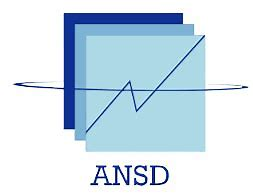
\includegraphics[width=4cm]{LOGO2.JPG} \\[0.1cm] 
        
        \textbf{\large Agence Nationale de la Statistique et de la Démographie}\\[0.2cm]
        
        
\includegraphics[width=4cm]{LOGO1.JPG} \\[0.1cm]  
        
        \textbf{\large École Nationale de la Statistique et de l'Analyse Économique}\\[0.4cm]
        
        \textbf{\LARGE A LA DECOUVERTE DE GTSUMMARY}\\[0.3cm]
        \textbf{\Huge \color{orange} \textsf{Illustration avec la base EHCVM 2021 de la Côte d'Ivoire}}\\[0.2cm]
        \rule{\linewidth}{0.2mm} \\[0.5cm]
        
        \begin{minipage}{0.5\textwidth}
    \begin{flushleft} \large
        \emph{\textsf{Rédigé par :}}\\
        \textbf{NGUEMFOUO NGOUMTSA Célina}\\
        \textit{Élève Ingénieure Statisticienne Économiste}
    \end{flushleft}
\end{minipage}
        \hfill
        \begin{minipage}{0.4\textwidth}
            \begin{flushright} \large
                \emph{\textsf{Sous la supervision de :}} \\
                \textbf{M. Aboubacar HEMA}\\
                \textit{Data analyst}
            \end{flushright}
        \end{minipage}

        \vfill

        {\large \textsf{Année scolaire : 2024/2025}}\\[0.5cm]
        
    \end{center}
\end{titlepage}

\phantomsection
\section*{Avant-propos}
\addcontentsline{toc}{section}{Avant-propos}

Dans un monde en constante évolution, le rôle des Ingénieurs
Statisticiens Économistes (ISE) est devenu indispensable pour répondre
aux enjeux complexes des sociétés modernes. Leur expertise en matière de
collecte, d'analyse et d'interprétation des données permet aux décideurs
publics et privés de mieux comprendre les dynamiques économiques,
sociales et démographiques, et de prendre des décisions éclairées. Grâce
à leur formation polyvalente, les ISE contribuent de manière décisive à
l'élaboration et à l'évaluation des politiques publiques, ainsi qu'au
développement de stratégies économiques efficaces.

C'est dans ce cadre que l'École nationale de la Statistique et de
l'Analyse économique Pierre Ndiaye (ENSAE) du Sénégal s'est imposée
comme l'un des principaux établissements de formation en Afrique
francophone. L'ENSAE offre plusieurs parcours de formation spécialisés
dans la statistique et l'économie appliquée, avec des filières comme :

\begin{itemize}
\tightlist
\item
  \textbf{Les Analystes Statisticiens (AS)} : une formation de trois
  ans, qui forme des techniciens en statistique capables de traiter et
  d'analyser des données à des fins variées.
\item
  \textbf{Les Ingénieurs Statisticiens Économistes (ISE)} : un cycle
  court de trois ans, et un cycle long de cinq ans, qui offre une
  formation approfondie à ceux qui souhaitent devenir des cadres
  spécialisés dans l'analyse statistique et économique.
\end{itemize}

L'accès à l'ENSAE est soumis à un concours rigoureux ouvert aux
étudiants détenteurs du baccalauréat ou d'un diplôme universitaire selon
le niveau d'admission. De plus, l'école propose des bourses pour les
étudiants méritants, facilitant ainsi l'accès à une formation
d'excellence, tant pour les étudiants sénégalais que pour ceux venant
d'autres pays africains francophones. En tant que membre du Réseau des
Écoles Africaines de la Statistique, l'ENSAE collabore étroitement avec
d'autres institutions prestigieuses comme l'Institut Sous-Régional de
Statistique et d'Économie Appliquée (ISSEA) au Cameroun et l'École
Nationale Supérieure de Statistique et d'Économie Appliquée (ENSEA) en
Côte d'Ivoire. Ce réseau permet d'harmoniser les programmes de formation
et d'offrir aux élèves une reconnaissance internationale de leurs
compétences.

Durant leur cursus, les étudiants de la filière ISE réalisent de
nombreux rapports pour leur permettre d'appliquer les concepts et de se
familiariser avec leurs outils de travail. Le présent rapport s'inscrit
dans cette démarche, et a pour thème \textbf{« A la découverte du
package gtsummary : Illustration avec la base EHCVM 2021 de la Côte
d'Ivoire »}.

\newpage

\phantomsection
\section*{Sommaire}
\addcontentsline{toc}{section}{Sommaire}

\setcounter{tocdepth}{1}
\tableofcontents

\newpage

\phantomsection
\section*{Résumé}
\addcontentsline{toc}{section}{Résumé}

Ce rapport explore l'utilisation du package gtsummary dans le cadre de
l'analyse statistique descriptive, en s'appuyant sur les données de
l'EHCVM 2021 de la Côte d'Ivoire. L'objectif est de montrer comment cet
outil facilite la génération de tableaux synthétiques et permet une
visualisation claire des statistiques descriptives. Après une
présentation du package et des données, nous illustrons les
fonctionnalités de la fonction tbl\_summary, qui permet de résumer
efficacement les variables d'un jeu de données. À travers des exemples
concrets, nous mettons en évidence la simplicité et la puissance de
gtsummary, notamment pour automatiser la production de rapports
statistiques. Ce travail s'inscrit dans une démarche plus large
d'amélioration des outils d'analyse de données, essentielle pour les
statisticiens et économistes en quête d'efficacité et de
reproductibilité.

\newpage

\phantomsection
\section*{Introduction}
\addcontentsline{toc}{section}{Introduction}

Dans le cadre de l'analyse des données, les ingénieurs statisticiens
économistes doivent extraire rapidement des informations pertinentes à
partir de vastes ensembles de données. L'une des premières étapes
exploratoires consiste à générer des résumés statistiques (summary),
permettant d'identifier les tendances générales, et d'obtenir une vision
synthétique des données avant d'engager des analyses plus approfondies.
Cette étape facilite la compréhension des distributions, la détection
des erreurs potentielles et l'adaptation des méthodes d'analyse. Les
fonctions classiques de R, comme \emph{summary()}, permettent d'obtenir
des statistiques descriptives de base. Cependant, elles présentent
plusieurs limites :

\begin{itemize}
\item
  Elles sont souvent générales et ne permettent pas d'obtenir des
  résumés adaptés à des types de données spécifiques (textes, facteurs,
  valeurs manquantes).
\item
  Elles manquent de flexibilité pour afficher des statistiques avancées
  comme l'asymétrie, l'aplatissement, ou des quantiles personnalisés.
\item
  Leur présentation n'est pas toujours optimisée pour l'interprétation
  et l'exportation des résultats.
\end{itemize}

Ce rapport vise à explorer le package \textbf{gtsummary}, qui fournit
des fonctions plus complètes et adaptées pour générer des résumés
statistiques avancés. Nous allons détailler son fonctionnement et
illustrer ses principales fonctionnalités à travers des exemples
concrets. Afin de repondre à cet objectif, notre rapport s'articulera en
2 chapitres. Le premier fera une brève présentation du package
\textbf{gtsummary} et de l'\textbf{EHCVM}, et le second s'attardera en
particulier sur la fonction \textbf{tbl\_summary} du package.

\newpage

\phantomsection
\section*{Chapitre 1 : présentation du package et de l'EHCVM}
\addcontentsline{toc}{section}{Chapitre 1 : présentation du package et de l'EHCVM}

\subsection{I. Présentation du package
gtsummary}\label{i.-pruxe9sentation-du-package-gtsummary}

Le package \textbf{gtsummary} est une extension de R conçue pour
faciliter la création de tableaux de synthèse et de rapports
statistiques bien structurés. Il est particulièrement utilisé en
biostatistique et en analyse de données pour produire des résumés
descriptifs, des comparaisons de groupes et des résultats de modèles
statistiques sous un format clair et lisible. Développé pour être
compatible avec des outils de présentation comme gt, flextable et
kableExtra, gtsummary permet d'obtenir des tableaux prêts à être
exportés dans des documents professionnels (Word, PDF, HTML). Il
s'intègre parfaitement avec les pipelines de tidyverse, notamment dplyr,
facilitant ainsi l'automatisation des analyses.

L'objectif principal de gtsummary est de simplifier la génération de
tableaux statistiques tout en garantissant une présentation soignée et
adaptée aux rapports scientifiques, une compatibilité avec plusieurs
formats d'exportation (HTML, Word, LaTeX), ainsi qu'une intégration
fluide avec dplyr pour un usage efficace dans les flux de travail en R.

Le package gtsummary propose plusieurs fonctions clés :

\begin{itemize}
\item
  \textbf{tbl\_summary() :} Génère un tableau de statistiques
  descriptives pour un jeu de données.
\item
  \textbf{tbl\_regression() :} Produit des tableaux de résultats pour
  les modèles de régression (linéaire, logistique, etc.).
\item
  \textbf{tbl\_compare() :} Compare des statistiques entre plusieurs
  groupes.
\item
  \textbf{tbl\_merge() :} Fusionne plusieurs tableaux gtsummary.
\item
  \textbf{as\_flextable() et as\_gt() :} Convertit les tableaux pour une
  personnalisation avancée et une meilleure exportation.
\end{itemize}

Dans la suite du rapport, nous nous concentrerons sur la fonction
\textbf{tbl\_summary} et de ses paramètres. Pour l'illusration, nous
utiliserons les bases \emph{ménages} et \emph{welfare} de l'EHCVM en
Côte d'Ivoire.

\newpage

\subsection{II. Présentation de
l'EHCVM}\label{ii.-pruxe9sentation-de-lehcvm}

L'\textbf{Enquête Harmonisée sur les Conditions de Vie des Ménages}
(EHCVM) est une initiative régionale menée dans plusieurs pays de
l'UEMOA, dont la \textbf{Côte d'Ivoire}, dans le but de produire des
données comparables sur le bien-être des ménages. Cette enquête
s'inscrit dans un cadre d'harmonisation des statistiques de la pauvreté
et des conditions de vie afin d'améliorer l'élaboration et l'évaluation
des politiques publiques.

L'EHCVM vise à fournir des informations détaillées sur :

\begin{itemize}
\item
  \textbf{Les conditions de vie des ménages} : accès aux services de
  base, logement, éducation, emploi.
\item
  \textbf{La consommation et la pauvreté} : estimation des dépenses des
  ménages pour calculer les indicateurs de bien-être économique.
\item
  \textbf{Les inégalités et la vulnérabilité} : analyse des écarts entre
  différents groupes sociaux et géographiques.
\item
  \textbf{L'impact des politiques publiques} : suivi des stratégies
  nationales de lutte contre la pauvreté et le développement humain.
\end{itemize}

L'enquête repose sur un échantillonnage représentatif au niveau
national, couvrant les zones urbaines et rurales. Les données sont
collectées à l'aide de questionnaires détaillés adressés aux ménages,
permettant d'analyser le profil sociodémographique des ménages, leur
accès aux infrastructures et services sociaux, leurs revenus, dépenses
et stratégies de subsistance.

Parmi les différentes bases de l'EHCVM, deux bases essentielles seront
utilisées dans cette analyse :

\begin{itemize}
\item
  \textbf{La base ``ménage''} : Contient les informations générales sur
  les ménages (composition, logement, accès aux services).
\item
  \textbf{La base ``welfare''} : Fournit des indicateurs clés sur la
  consommation, la pauvreté et le bien-être économique des ménages. Ces
  bases de données permettent une exploration approfondie des dynamiques
  socioéconomiques en Côte d'Ivoire et constituent des sources
  précieuses pour les analyses quantitatives.
\end{itemize}

\newpage

\phantomsection
\section*{Chapitre 2 : fontion tbl summary}
\addcontentsline{toc}{section}{Chapitre 2 : fontion tbl summary}

\subsection{I. Base ménage}\label{i.-base-muxe9nage}

la base ménage a d'abord été importée. Pour ce faire, le package
\textbf{haven} a été utilisé. Il s'agit d'un fichier .dta.

\begin{Shaded}
\begin{Highlighting}[]
\FunctionTok{library}\NormalTok{(haven)}
\NormalTok{menage }\OtherTok{\textless{}{-}} \FunctionTok{read\_dta}\NormalTok{(}
  \StringTok{"CIV\_2021\_EHCVM\_Stata/ehcvm\_menage\_civ2021.dta"}\NormalTok{)}
\end{Highlighting}
\end{Shaded}

Voici les premières lignes de la base

\begin{Shaded}
\begin{Highlighting}[]
\FunctionTok{library}\NormalTok{(knitr)}
\FunctionTok{kable}\NormalTok{(}\FunctionTok{head}\NormalTok{(menage[, }\DecValTok{1}\SpecialCharTok{:}\DecValTok{10}\NormalTok{]))}
\end{Highlighting}
\end{Shaded}

\begin{longtable}[]{@{}
  >{\raggedright\arraybackslash}p{(\columnwidth - 18\tabcolsep) * \real{0.1290}}
  >{\raggedleft\arraybackslash}p{(\columnwidth - 18\tabcolsep) * \real{0.0806}}
  >{\raggedleft\arraybackslash}p{(\columnwidth - 18\tabcolsep) * \real{0.1129}}
  >{\raggedleft\arraybackslash}p{(\columnwidth - 18\tabcolsep) * \real{0.1129}}
  >{\raggedleft\arraybackslash}p{(\columnwidth - 18\tabcolsep) * \real{0.0968}}
  >{\raggedleft\arraybackslash}p{(\columnwidth - 18\tabcolsep) * \real{0.0968}}
  >{\raggedleft\arraybackslash}p{(\columnwidth - 18\tabcolsep) * \real{0.0645}}
  >{\raggedleft\arraybackslash}p{(\columnwidth - 18\tabcolsep) * \real{0.0806}}
  >{\raggedleft\arraybackslash}p{(\columnwidth - 18\tabcolsep) * \real{0.0645}}
  >{\raggedleft\arraybackslash}p{(\columnwidth - 18\tabcolsep) * \real{0.1613}}@{}}
\toprule\noalign{}
\begin{minipage}[b]{\linewidth}\raggedright
country
\end{minipage} & \begin{minipage}[b]{\linewidth}\raggedleft
hhid
\end{minipage} & \begin{minipage}[b]{\linewidth}\raggedleft
grappe
\end{minipage} & \begin{minipage}[b]{\linewidth}\raggedleft
menage
\end{minipage} & \begin{minipage}[b]{\linewidth}\raggedleft
vague
\end{minipage} & \begin{minipage}[b]{\linewidth}\raggedleft
logem
\end{minipage} & \begin{minipage}[b]{\linewidth}\raggedleft
mur
\end{minipage} & \begin{minipage}[b]{\linewidth}\raggedleft
toit
\end{minipage} & \begin{minipage}[b]{\linewidth}\raggedleft
sol
\end{minipage} & \begin{minipage}[b]{\linewidth}\raggedleft
eauboi\_ss
\end{minipage} \\
\midrule\noalign{}
\endhead
\bottomrule\noalign{}
\endlastfoot
& 101 & NA & NA & NA & NA & NA & NA & NA & NA \\
CIV & 102 & 1 & 2 & 1 & 3 & 1 & 1 & 1 & 1 \\
CIV & 103 & 1 & 3 & 1 & 3 & 1 & 1 & 1 & 1 \\
CIV & 104 & 1 & 4 & 1 & 4 & 1 & 1 & 1 & 1 \\
CIV & 105 & 1 & 5 & 1 & 3 & 1 & 1 & 1 & 1 \\
CIV & 106 & 1 & 6 & 1 & 3 & 1 & 1 & 1 & 1 \\
\end{longtable}

Visualisons à présent un summary des variables \emph{logem, toit} et
\emph{sol}.

Pour cela, il faut charger la librairie \textbf{gtsummary}.

\begin{Shaded}
\begin{Highlighting}[]
\FunctionTok{library}\NormalTok{(gtsummary)}
\FunctionTok{suppressMessages}\NormalTok{(}
\NormalTok{  menage }\SpecialCharTok{\%\textgreater{}\%} \FunctionTok{select}\NormalTok{(logem,toit,sol) }\SpecialCharTok{\%\textgreater{}\%} \FunctionTok{tbl\_summary}\NormalTok{()}
\NormalTok{  )}
\end{Highlighting}
\end{Shaded}

\begin{table}[!t]
\fontsize{12.0pt}{14.4pt}\selectfont
\begin{tabular*}{\linewidth}{@{\extracolsep{\fill}}lc}
\toprule
\textbf{Characteristic} & \textbf{N = 13,863}\textsuperscript{\textit{1}} \\ 
\midrule\addlinespace[2.5pt]
Occupation logement &  \\ 
    1 & 2,844 (22\%) \\ 
    2 & 4,508 (35\%) \\ 
    3 & 2,702 (21\%) \\ 
    4 & 2,906 (22\%) \\ 
    9 & 5 (<0.1\%) \\ 
    Unknown & 898 \\ 
toit en materiaux definitifs &  \\ 
    0 & 1,337 (10\%) \\ 
    1 & 11,628 (90\%) \\ 
    Unknown & 898 \\ 
Sol en materiaux definitifs &  \\ 
    0 & 1,736 (13\%) \\ 
    1 & 11,229 (87\%) \\ 
    Unknown & 898 \\ 
\bottomrule
\end{tabular*}
\begin{minipage}{\linewidth}
\textsuperscript{\textit{1}}n (\%)\\
\end{minipage}
\end{table}

\newpage

Affichons à présent les modalités des variables:

\begin{Shaded}
\begin{Highlighting}[]
\NormalTok{menage }\SpecialCharTok{\%\textgreater{}\%}
\NormalTok{  labelled}\SpecialCharTok{::}\FunctionTok{to\_factor}\NormalTok{() }\SpecialCharTok{\%\textgreater{}\%}
  \FunctionTok{select}\NormalTok{(logem,toit,sol) }\SpecialCharTok{\%\textgreater{}\%}
  \FunctionTok{tbl\_summary}\NormalTok{()}
\end{Highlighting}
\end{Shaded}

\begin{table}[!t]
\fontsize{12.0pt}{14.4pt}\selectfont
\begin{tabular*}{\linewidth}{@{\extracolsep{\fill}}lc}
\toprule
\textbf{Characteristic} & \textbf{N = 13,863}\textsuperscript{\textit{1}} \\ 
\midrule\addlinespace[2.5pt]
Occupation logement &  \\ 
    Proprietaire titre & 2,844 (22\%) \\ 
    Proprietaire sans titre & 4,508 (35\%) \\ 
    Locataire & 2,702 (21\%) \\ 
    Autre & 2,906 (22\%) \\ 
    9 & 5 (<0.1\%) \\ 
    Unknown & 898 \\ 
toit en materiaux definitifs &  \\ 
    Non & 1,337 (10\%) \\ 
    Oui & 11,628 (90\%) \\ 
    Unknown & 898 \\ 
Sol en materiaux definitifs &  \\ 
    Non & 1,736 (13\%) \\ 
    Oui & 11,229 (87\%) \\ 
    Unknown & 898 \\ 
\bottomrule
\end{tabular*}
\begin{minipage}{\linewidth}
\textsuperscript{\textit{1}}n (\%)\\
\end{minipage}
\end{table}

\newpage

Attribuons à présent des labels aux différentes variables sélectionnées

\begin{Shaded}
\begin{Highlighting}[]
\NormalTok{menage }\SpecialCharTok{\%\textgreater{}\%}
\NormalTok{  labelled}\SpecialCharTok{::}\FunctionTok{to\_factor}\NormalTok{() }\SpecialCharTok{\%\textgreater{}\%}
  \FunctionTok{select}\NormalTok{(logem,toit,sol) }\SpecialCharTok{\%\textgreater{}\%}
  \FunctionTok{tbl\_summary}\NormalTok{(}
    \AttributeTok{label=}\FunctionTok{list}\NormalTok{(logem}\SpecialCharTok{\textasciitilde{}}\StringTok{"Type de logement du CM"}\NormalTok{,}
\NormalTok{               toit}\SpecialCharTok{\textasciitilde{}}\StringTok{"Type de toit de la maison du CM"}\NormalTok{,}
\NormalTok{               sol}\SpecialCharTok{\textasciitilde{}}\StringTok{"Yype de sol de la maison du CM"}\NormalTok{))}
\end{Highlighting}
\end{Shaded}

\begin{table}[!t]
\fontsize{12.0pt}{14.4pt}\selectfont
\begin{tabular*}{\linewidth}{@{\extracolsep{\fill}}lc}
\toprule
\textbf{Characteristic} & \textbf{N = 13,863}\textsuperscript{\textit{1}} \\ 
\midrule\addlinespace[2.5pt]
Type de logement du CM &  \\ 
    Proprietaire titre & 2,844 (22\%) \\ 
    Proprietaire sans titre & 4,508 (35\%) \\ 
    Locataire & 2,702 (21\%) \\ 
    Autre & 2,906 (22\%) \\ 
    9 & 5 (<0.1\%) \\ 
    Unknown & 898 \\ 
Type de toit de la maison du CM &  \\ 
    Non & 1,337 (10\%) \\ 
    Oui & 11,628 (90\%) \\ 
    Unknown & 898 \\ 
Yype de sol de la maison du CM &  \\ 
    Non & 1,736 (13\%) \\ 
    Oui & 11,229 (87\%) \\ 
    Unknown & 898 \\ 
\bottomrule
\end{tabular*}
\begin{minipage}{\linewidth}
\textsuperscript{\textit{1}}n (\%)\\
\end{minipage}
\end{table}

\newpage

Modifions à présent le titre du tableau

\begin{Shaded}
\begin{Highlighting}[]
\NormalTok{menage }\SpecialCharTok{\%\textgreater{}\%}\NormalTok{ labelled}\SpecialCharTok{::}\FunctionTok{to\_factor}\NormalTok{() }\SpecialCharTok{\%\textgreater{}\%}
  \FunctionTok{select}\NormalTok{(logem,toit,sol) }\SpecialCharTok{\%\textgreater{}\%}
  \FunctionTok{tbl\_summary}\NormalTok{(}
    \AttributeTok{label=}\FunctionTok{list}\NormalTok{(logem}\SpecialCharTok{\textasciitilde{}}\StringTok{"Type de logement du CM"}\NormalTok{,}
\NormalTok{               toit}\SpecialCharTok{\textasciitilde{}}\StringTok{"Type de toit de la maison du CM"}\NormalTok{,}
\NormalTok{               sol}\SpecialCharTok{\textasciitilde{}}\StringTok{"Type de sol de la maison du CM"}\NormalTok{)) }\SpecialCharTok{\%\textgreater{}\%}
  \FunctionTok{modify\_header}\NormalTok{(}\AttributeTok{label=}\StringTok{"Caractéristiques de l\textquotesingle{}habitat du CM"}\NormalTok{)}
\end{Highlighting}
\end{Shaded}

\begin{table}[!t]
\fontsize{12.0pt}{14.4pt}\selectfont
\begin{tabular*}{\linewidth}{@{\extracolsep{\fill}}lc}
\toprule
Caractéristiques de l'habitat du CM & \textbf{N = 13,863}\textsuperscript{\textit{1}} \\ 
\midrule\addlinespace[2.5pt]
Type de logement du CM &  \\ 
    Proprietaire titre & 2,844 (22\%) \\ 
    Proprietaire sans titre & 4,508 (35\%) \\ 
    Locataire & 2,702 (21\%) \\ 
    Autre & 2,906 (22\%) \\ 
    9 & 5 (<0.1\%) \\ 
    Unknown & 898 \\ 
Type de toit de la maison du CM &  \\ 
    Non & 1,337 (10\%) \\ 
    Oui & 11,628 (90\%) \\ 
    Unknown & 898 \\ 
Type de sol de la maison du CM &  \\ 
    Non & 1,736 (13\%) \\ 
    Oui & 11,229 (87\%) \\ 
    Unknown & 898 \\ 
\bottomrule
\end{tabular*}
\begin{minipage}{\linewidth}
\textsuperscript{\textit{1}}n (\%)\\
\end{minipage}
\end{table}

Considérons à présent les variables \emph{superf, grosrum} et
\emph{petitrum} Comme il s'agit de variable numériques, le paramètre
\textbf{statistic} a été ajouté pour visualiser la \textbf{moyenne}
(mean) et l'écartype (sd).

\begin{Shaded}
\begin{Highlighting}[]
\NormalTok{menage }\SpecialCharTok{\%\textgreater{}\%}
\NormalTok{  labelled}\SpecialCharTok{::}\FunctionTok{to\_factor}\NormalTok{() }\SpecialCharTok{\%\textgreater{}\%}
  \FunctionTok{select}\NormalTok{(superf,grosrum,petitrum) }\SpecialCharTok{\%\textgreater{}\%}
  \FunctionTok{tbl\_summary}\NormalTok{(}
    \AttributeTok{label=}\FunctionTok{list}\NormalTok{(superf}\SpecialCharTok{\textasciitilde{}}\StringTok{"Superficie agricole en moyenne par ménage"}\NormalTok{,}
\NormalTok{               grosrum}\SpecialCharTok{\textasciitilde{}}\StringTok{"Nombre de gros ruminants en moyenne par ménage"}\NormalTok{,}
\NormalTok{               petitrum}\SpecialCharTok{\textasciitilde{}}\StringTok{"Nombre de petits ruminants en moyenne par ménage"}\NormalTok{),}
    \AttributeTok{statistic =} \FunctionTok{list}\NormalTok{(superf}\SpecialCharTok{\textasciitilde{}}\StringTok{"\{mean\}(\{sd\})"}\NormalTok{,}
\NormalTok{                     grosrum}\SpecialCharTok{\textasciitilde{}}\StringTok{"\{mean\}(\{sd\})"}\NormalTok{,}
\NormalTok{                     petitrum}\SpecialCharTok{\textasciitilde{}}\StringTok{"\{mean\}(\{sd\})"}\NormalTok{)) }\SpecialCharTok{\%\textgreater{}\%}
  \FunctionTok{modify\_header}\NormalTok{(}\AttributeTok{label=}\StringTok{"Caractéristiques de l\textquotesingle{}habitat du CM"}\NormalTok{)}
\end{Highlighting}
\end{Shaded}

\begin{table}[!t]
\fontsize{12.0pt}{14.4pt}\selectfont
\begin{tabular*}{\linewidth}{@{\extracolsep{\fill}}lc}
\toprule
Caractéristiques de l'habitat du CM & \textbf{N = 13,863}\textsuperscript{\textit{1}} \\ 
\midrule\addlinespace[2.5pt]
Superficie agricole en moyenne par ménage & 24,660,570(1,441,480,913) \\ 
    Unknown & 898 \\ 
Nombre de gros ruminants en moyenne par ménage & 0.7405(9.1305) \\ 
    Unknown & 898 \\ 
Nombre de petits ruminants en moyenne par ménage & 0.93(3.83) \\ 
    Unknown & 898 \\ 
\bottomrule
\end{tabular*}
\begin{minipage}{\linewidth}
\textsuperscript{\textit{1}}Mean(SD)\\
\end{minipage}
\end{table}

les valeurs présentes dans le tableau comme indiqué dans la dernière
ligne sont les moyennes et entre parenthèse l'écart-type pour chacune
des variables. On constate la présence de valeurs manquantes.

Le code suivant permet de toujours les afficher:

\begin{Shaded}
\begin{Highlighting}[]
\NormalTok{menage }\SpecialCharTok{\%\textgreater{}\%}
\NormalTok{  labelled}\SpecialCharTok{::}\FunctionTok{to\_factor}\NormalTok{() }\SpecialCharTok{\%\textgreater{}\%}
  \FunctionTok{select}\NormalTok{(superf,grosrum,petitrum) }\SpecialCharTok{\%\textgreater{}\%}
  \FunctionTok{tbl\_summary}\NormalTok{(}
    \AttributeTok{label=}\FunctionTok{list}\NormalTok{(superf}\SpecialCharTok{\textasciitilde{}}\StringTok{"Superficie agricole en moyenne par ménage"}\NormalTok{,}
\NormalTok{               grosrum}\SpecialCharTok{\textasciitilde{}}\StringTok{"Nombre de gros ruminants en moyenne par ménage"}\NormalTok{,}
\NormalTok{               petitrum}\SpecialCharTok{\textasciitilde{}}\StringTok{"Nombre de petits ruminants en moyenne par ménage"}\NormalTok{),}
    \AttributeTok{statistic =} \FunctionTok{list}\NormalTok{(superf}\SpecialCharTok{\textasciitilde{}}\StringTok{"\{mean\}(\{sd\})"}\NormalTok{,}
\NormalTok{                     grosrum}\SpecialCharTok{\textasciitilde{}}\StringTok{"\{mean\}(\{sd\})"}\NormalTok{,}
\NormalTok{                     petitrum}\SpecialCharTok{\textasciitilde{}}\StringTok{"\{mean\}(\{sd\})"}\NormalTok{),}
    \AttributeTok{missing=}\StringTok{"always"}\NormalTok{) }\SpecialCharTok{\%\textgreater{}\%}
  \FunctionTok{modify\_header}\NormalTok{(}\AttributeTok{label=}\StringTok{"Caractéristiques de l\textquotesingle{}habitat du CM"}\NormalTok{)}
\end{Highlighting}
\end{Shaded}

\begin{table}[!t]
\fontsize{12.0pt}{14.4pt}\selectfont
\begin{tabular*}{\linewidth}{@{\extracolsep{\fill}}lc}
\toprule
Caractéristiques de l'habitat du CM & \textbf{N = 13,863}\textsuperscript{\textit{1}} \\ 
\midrule\addlinespace[2.5pt]
Superficie agricole en moyenne par ménage & 24,660,570(1,441,480,913) \\ 
    Unknown & 898 \\ 
Nombre de gros ruminants en moyenne par ménage & 0.7405(9.1305) \\ 
    Unknown & 898 \\ 
Nombre de petits ruminants en moyenne par ménage & 0.93(3.83) \\ 
    Unknown & 898 \\ 
\bottomrule
\end{tabular*}
\begin{minipage}{\linewidth}
\textsuperscript{\textit{1}}Mean(SD)\\
\end{minipage}
\end{table}

On a également la possibilté de renommer les valeurs manquantes.

\begin{Shaded}
\begin{Highlighting}[]
\NormalTok{menage }\SpecialCharTok{\%\textgreater{}\%}
\NormalTok{  labelled}\SpecialCharTok{::}\FunctionTok{to\_factor}\NormalTok{() }\SpecialCharTok{\%\textgreater{}\%}
  \FunctionTok{select}\NormalTok{(superf,grosrum,petitrum) }\SpecialCharTok{\%\textgreater{}\%}
  \FunctionTok{tbl\_summary}\NormalTok{(}
    \AttributeTok{label=}\FunctionTok{list}\NormalTok{(superf}\SpecialCharTok{\textasciitilde{}}\StringTok{"Superficie agricole en moyenne par ménage"}\NormalTok{,}
\NormalTok{               grosrum}\SpecialCharTok{\textasciitilde{}}\StringTok{"Nombre de gros ruminants en moyenne par ménage"}\NormalTok{,}
\NormalTok{               petitrum}\SpecialCharTok{\textasciitilde{}}\StringTok{"Nombre de petits ruminants en moyenne par ménage"}\NormalTok{),}
    \AttributeTok{statistic =} \FunctionTok{list}\NormalTok{(superf}\SpecialCharTok{\textasciitilde{}}\StringTok{"\{mean\}(\{sd\})"}\NormalTok{,}
\NormalTok{                     grosrum}\SpecialCharTok{\textasciitilde{}}\StringTok{"\{mean\}(\{sd\})"}\NormalTok{,}
\NormalTok{                     petitrum}\SpecialCharTok{\textasciitilde{}}\StringTok{"\{mean\}(\{sd\})"}\NormalTok{),}
    \AttributeTok{missing=}\StringTok{"always"}\NormalTok{,}
    \AttributeTok{missing\_text =} \StringTok{"Valeurs manquantes"}\NormalTok{) }\SpecialCharTok{\%\textgreater{}\%}
  \FunctionTok{modify\_header}\NormalTok{(}\AttributeTok{label=}\StringTok{"Caractéristiques de l\textquotesingle{}habitat du CM"}\NormalTok{)}
\end{Highlighting}
\end{Shaded}

\begin{table}[!t]
\fontsize{12.0pt}{14.4pt}\selectfont
\begin{tabular*}{\linewidth}{@{\extracolsep{\fill}}lc}
\toprule
Caractéristiques de l'habitat du CM & \textbf{N = 13,863}\textsuperscript{\textit{1}} \\ 
\midrule\addlinespace[2.5pt]
Superficie agricole en moyenne par ménage & 24,660,570(1,441,480,913) \\ 
    Valeurs manquantes & 898 \\ 
Nombre de gros ruminants en moyenne par ménage & 0.7405(9.1305) \\ 
    Valeurs manquantes & 898 \\ 
Nombre de petits ruminants en moyenne par ménage & 0.93(3.83) \\ 
    Valeurs manquantes & 898 \\ 
\bottomrule
\end{tabular*}
\begin{minipage}{\linewidth}
\textsuperscript{\textit{1}}Mean(SD)\\
\end{minipage}
\end{table}

On peut en outre choisir le nombre de chiffres après la virgule.
Choisissons aucun chiffre après la virgule :

\begin{Shaded}
\begin{Highlighting}[]
\NormalTok{menage }\SpecialCharTok{\%\textgreater{}\%}
\NormalTok{  labelled}\SpecialCharTok{::}\FunctionTok{to\_factor}\NormalTok{() }\SpecialCharTok{\%\textgreater{}\%}
  \FunctionTok{select}\NormalTok{(superf,grosrum,petitrum) }\SpecialCharTok{\%\textgreater{}\%}
  \FunctionTok{tbl\_summary}\NormalTok{(}
    \AttributeTok{label=}\FunctionTok{list}\NormalTok{(superf}\SpecialCharTok{\textasciitilde{}}\StringTok{"Superficie agricole en moyenne par ménage"}\NormalTok{,}
\NormalTok{               grosrum}\SpecialCharTok{\textasciitilde{}}\StringTok{"Nombre de gros ruminants en moyenne par ménage"}\NormalTok{,}
\NormalTok{               petitrum}\SpecialCharTok{\textasciitilde{}}\StringTok{"Nombre de petits ruminants en moyenne par ménage"}\NormalTok{),}
    \AttributeTok{statistic =} \FunctionTok{list}\NormalTok{(superf}\SpecialCharTok{\textasciitilde{}}\StringTok{"\{mean\}(\{sd\})"}\NormalTok{,}
\NormalTok{                     grosrum}\SpecialCharTok{\textasciitilde{}}\StringTok{"\{mean\}(\{sd\})"}\NormalTok{,}
\NormalTok{                     petitrum}\SpecialCharTok{\textasciitilde{}}\StringTok{"\{mean\}(\{sd\})"}\NormalTok{),}
    \AttributeTok{digits =} \FunctionTok{everything}\NormalTok{()}\SpecialCharTok{\textasciitilde{}}\FunctionTok{c}\NormalTok{(}\DecValTok{0}\NormalTok{,}\DecValTok{0}\NormalTok{,}\DecValTok{0}\NormalTok{),}
    \AttributeTok{missing=}\StringTok{"always"}\NormalTok{,}
    \AttributeTok{missing\_text =} \StringTok{"Valeurs manquantes"}\NormalTok{) }\SpecialCharTok{\%\textgreater{}\%}
  \FunctionTok{modify\_header}\NormalTok{(}\AttributeTok{label=}\StringTok{"Caractéristiques de l\textquotesingle{}habitat du CM"}\NormalTok{)}
\end{Highlighting}
\end{Shaded}

\begin{table}[!t]
\fontsize{12.0pt}{14.4pt}\selectfont
\begin{tabular*}{\linewidth}{@{\extracolsep{\fill}}lc}
\toprule
Caractéristiques de l'habitat du CM & \textbf{N = 13,863}\textsuperscript{\textit{1}} \\ 
\midrule\addlinespace[2.5pt]
Superficie agricole en moyenne par ménage & 24,660,570(1,441,480,913) \\ 
    Valeurs manquantes & 898 \\ 
Nombre de gros ruminants en moyenne par ménage & 1(9) \\ 
    Valeurs manquantes & 898 \\ 
Nombre de petits ruminants en moyenne par ménage & 1(4) \\ 
    Valeurs manquantes & 898 \\ 
\bottomrule
\end{tabular*}
\begin{minipage}{\linewidth}
\textsuperscript{\textit{1}}Mean(SD)\\
\end{minipage}
\end{table}

\newpage

\subsection{II. Base welfare}\label{ii.-base-welfare}

Commençons par charger la base en question.

\begin{Shaded}
\begin{Highlighting}[]
\FunctionTok{library}\NormalTok{(haven)}
\NormalTok{welfare }\OtherTok{\textless{}{-}} \FunctionTok{read\_dta}\NormalTok{(}
  \StringTok{"CIV\_2021\_EHCVM\_Stata/ehcvm\_welfare\_civ2021.dta"}
\NormalTok{  )}
\end{Highlighting}
\end{Shaded}

voici un aperçu de la base chargée :

\begin{Shaded}
\begin{Highlighting}[]
\FunctionTok{library}\NormalTok{(knitr)}
\FunctionTok{kable}\NormalTok{(}\FunctionTok{head}\NormalTok{(welfare[, }\DecValTok{1}\SpecialCharTok{:}\DecValTok{10}\NormalTok{]))}
\end{Highlighting}
\end{Shaded}

\begin{longtable}[]{@{}
  >{\raggedleft\arraybackslash}p{(\columnwidth - 18\tabcolsep) * \real{0.1045}}
  >{\raggedleft\arraybackslash}p{(\columnwidth - 18\tabcolsep) * \real{0.1045}}
  >{\raggedright\arraybackslash}p{(\columnwidth - 18\tabcolsep) * \real{0.1194}}
  >{\raggedleft\arraybackslash}p{(\columnwidth - 18\tabcolsep) * \real{0.0746}}
  >{\raggedleft\arraybackslash}p{(\columnwidth - 18\tabcolsep) * \real{0.0746}}
  >{\raggedleft\arraybackslash}p{(\columnwidth - 18\tabcolsep) * \real{0.0896}}
  >{\raggedright\arraybackslash}p{(\columnwidth - 18\tabcolsep) * \real{0.1642}}
  >{\raggedleft\arraybackslash}p{(\columnwidth - 18\tabcolsep) * \real{0.0597}}
  >{\raggedleft\arraybackslash}p{(\columnwidth - 18\tabcolsep) * \real{0.1045}}
  >{\raggedleft\arraybackslash}p{(\columnwidth - 18\tabcolsep) * \real{0.1045}}@{}}
\toprule\noalign{}
\begin{minipage}[b]{\linewidth}\raggedleft
grappe
\end{minipage} & \begin{minipage}[b]{\linewidth}\raggedleft
menage
\end{minipage} & \begin{minipage}[b]{\linewidth}\raggedright
country
\end{minipage} & \begin{minipage}[b]{\linewidth}\raggedleft
year
\end{minipage} & \begin{minipage}[b]{\linewidth}\raggedleft
hhid
\end{minipage} & \begin{minipage}[b]{\linewidth}\raggedleft
vague
\end{minipage} & \begin{minipage}[b]{\linewidth}\raggedright
month
\end{minipage} & \begin{minipage}[b]{\linewidth}\raggedleft
zae
\end{minipage} & \begin{minipage}[b]{\linewidth}\raggedleft
region
\end{minipage} & \begin{minipage}[b]{\linewidth}\raggedleft
milieu
\end{minipage} \\
\midrule\noalign{}
\endhead
\bottomrule\noalign{}
\endlastfoot
1 & 11 & CIV & 2021 & 111 & 1 & 2022-01-01 & 6 & 1 & 1 \\
1 & 27 & CIV & 2021 & 127 & 1 & 2022-02-01 & 6 & 1 & 1 \\
1 & 7 & CIV & 2021 & 107 & 1 & 2022-01-01 & 6 & 1 & 1 \\
1 & 8 & CIV & 2021 & 108 & 1 & 2022-01-01 & 6 & 1 & 1 \\
1 & 10 & CIV & 2021 & 110 & 1 & 2022-01-01 & 6 & 1 & 1 \\
1 & 9 & CIV & 2021 & 109 & 1 & 2022-01-01 & 6 & 1 & 1 \\
\end{longtable}

Faisons à présent un summary pour les variables hgender, hage, hmstat,
heduc, hdiploma. Seule la variable age est numérique, donc c'est
uniquement pour elle que le paramètre statistic (mean et sd) a été
défini. Les modalités ont été affichées, le titre du tableau renomé, le
nombre de chiffre après la virgule fixé, et les valeurs manquantes
affichées. Voici le résultat:

\begin{Shaded}
\begin{Highlighting}[]
\NormalTok{welfare }\SpecialCharTok{\%\textgreater{}\%}
\NormalTok{  labelled}\SpecialCharTok{::}\FunctionTok{to\_factor}\NormalTok{() }\SpecialCharTok{\%\textgreater{}\%}
  \FunctionTok{select}\NormalTok{(hgender, hage, hmstat, heduc, hdiploma) }\SpecialCharTok{\%\textgreater{}\%}
  \FunctionTok{tbl\_summary}\NormalTok{(}\AttributeTok{label=}\FunctionTok{list}\NormalTok{(hgender}\SpecialCharTok{\textasciitilde{}}\StringTok{"Genre du CM"}\NormalTok{,}
\NormalTok{                         hage}\SpecialCharTok{\textasciitilde{}}\StringTok{"Âge du CM"}\NormalTok{,}
\NormalTok{                         hmstat}\SpecialCharTok{\textasciitilde{}}\StringTok{"Situation matrimoniale du CM"}\NormalTok{,}
\NormalTok{                         heduc}\SpecialCharTok{\textasciitilde{}}\StringTok{"Niveau d\textquotesingle{}étude du CM"}\NormalTok{,}
\NormalTok{                         hdiploma}\SpecialCharTok{\textasciitilde{}}\StringTok{"Diplome le plus élevé"}\NormalTok{),}
              \AttributeTok{statistic =} \FunctionTok{list}\NormalTok{(hage}\SpecialCharTok{\textasciitilde{}}\StringTok{"\{mean\}(\{sd\})"}\NormalTok{),}
              \AttributeTok{digits =} \FunctionTok{everything}\NormalTok{()}\SpecialCharTok{\textasciitilde{}}\FunctionTok{c}\NormalTok{(}\DecValTok{0}\NormalTok{,}\DecValTok{0}\NormalTok{,}\DecValTok{0}\NormalTok{),}
              \AttributeTok{missing=}\StringTok{"always"}\NormalTok{,}
              \AttributeTok{missing\_text =} \StringTok{"Valeurs manquantes"}\NormalTok{)}\SpecialCharTok{\%\textgreater{}\%}
  \FunctionTok{modify\_header}\NormalTok{(}\AttributeTok{label=}\StringTok{"Caractéristiques du chef de ménage"}\NormalTok{)}
\end{Highlighting}
\end{Shaded}

\begin{table}[!t]
\fontsize{12.0pt}{14.4pt}\selectfont
\begin{tabular*}{\linewidth}{@{\extracolsep{\fill}}lc}
\toprule
Caractéristiques du chef de ménage & \textbf{N = 12,965}\textsuperscript{\textit{1}} \\ 
\midrule\addlinespace[2.5pt]
Genre du CM &  \\ 
    Masculin & 10,689 (82\%) \\ 
    Féminin & 2,276 (18\%) \\ 
    Valeurs manquantes & 0 \\ 
Âge du CM & 46(14) \\ 
    Valeurs manquantes & 0 \\ 
Situation matrimoniale du CM &  \\ 
    Célibataire & 1,907 (15\%) \\ 
    Marié(e) monogame & 7,171 (55\%) \\ 
    Marié(e) polygame & 1,656 (13\%) \\ 
    Union libre & 811 (6\%) \\ 
    Veuf(ve) & 1,078 (8\%) \\ 
    Divorcé(e) & 161 (1\%) \\ 
    Séparé & 181 (1\%) \\ 
    Valeurs manquantes & 0 \\ 
Niveau d'étude du CM &  \\ 
    Aucun & 7,444 (57\%) \\ 
    Maternelle & 3 (0\%) \\ 
    Primaire & 2,544 (20\%) \\ 
    Second. gl 1 & 1,409 (11\%) \\ 
    Second. tech. 1 & 36 (0\%) \\ 
    Second. gl 2 & 791 (6\%) \\ 
    Second. tech. 2 & 73 (1\%) \\ 
    Postsecondaire & 257 (2\%) \\ 
    Superieur & 407 (3\%) \\ 
    Valeurs manquantes & 1 \\ 
Diplome le plus élevé &  \\ 
    Aucun & 9,759 (75\%) \\ 
    cepe & 1,499 (12\%) \\ 
    bepc & 755 (6\%) \\ 
    cap & 35 (0\%) \\ 
    bt & 41 (0\%) \\ 
    bac & 339 (3\%) \\ 
    DEUG, DUT, BTS & 242 (2\%) \\ 
    Licence & 118 (1\%) \\ 
    Maitrise / Ingénieur des travaux & 89 (1\%) \\ 
    Master/DEA/DESS/Ingénieur de conception & 71 (1\%) \\ 
    Doctorat/Phd & 17 (0\%) \\ 
    Valeurs manquantes & 0 \\ 
\bottomrule
\end{tabular*}
\begin{minipage}{\linewidth}
\textsuperscript{\textit{1}}n (\%); Mean(SD)\\
\end{minipage}
\end{table}

\newpage

\phantomsection
\section*{Conclusion}
\addcontentsline{toc}{section}{Conclusion}

L'utilisation du package gtsummary s'avère être une solution efficace
pour la synthèse et la présentation des statistiques descriptives,
particulièrement dans le cadre de l'analyse d'enquêtes comme l'EHCVM
2021. Grâce à ses fonctionnalités intuitives, il permet de gagner du
temps et d'assurer une meilleure lisibilité des résultats. L'application
de tbl\_summary démontre qu'il est possible de produire des tableaux
complets et personnalisables avec un minimum d'effort, tout en
garantissant une présentation standardisée. Ce rapport met ainsi en
avant l'intérêt d'intégrer des outils comme gtsummary dans les pratiques
courantes des statisticiens, contribuant ainsi à une analyse plus rapide
et plus fiable des données.

\newpage

\phantomsection
\section*{Table de matières}
\addcontentsline{toc}{section}{Table de matières}

Avant-propos

Sommaire

Résumé

Introduction

Chapitre 1 : présentation du package et de l'EHCVM

I. Présentation du package gtsummary

\begin{enumerate}
\def\labelenumi{\Roman{enumi}.}
\setcounter{enumi}{1}
\tightlist
\item
  Présentation de l'EHCVM
\end{enumerate}

Chapitre 2 : fonction tbl summary

I. Base ménage

\begin{enumerate}
\def\labelenumi{\Roman{enumi}.}
\setcounter{enumi}{1}
\tightlist
\item
  Base welfare
\end{enumerate}

Conclusion

Table de matières

\end{document}
